\chapter{Desarrollo del Detector de Rostros y la Arquitectura de Red Neuronal Convolucional}

\section{Detección de Rostros}
En este trabajo se optó por utilizar como etapa inicial dentro de la fase de consultas a la red, la construcción de un detector de rostros, debido a que, al momento de desarrollar una aplicación orientada a las necesidades del mundo real, este no solo recibira como entrada imágenes que contengan exactamente el rostro de la persona, sino, imágenes con el cuerpo completo o algunas partes adicionales aparte del rostro. Sin embargo, en objetivo del trabajo es poder detectar la expresión facial de una persona, para lo cual, basta con tener como entrada a la red una imagen que delimite el rostro de la persona. De ahí, la necesidad de utilizar un algoritmo de detección de rostros para la extracción de la región de interes que posteriormente servira como entrada para la red neuronal convolucional encargada de reconocer la expresión facial correspondiente. La figura~\ref{fig:imagen_entrada} muestra un ejemplo de una imagen de entrada, en la cual, se puede observar detalles adicionales aparte del rostro(el sombrero y el fondo), los cuales no aportan carasteristicas relevantes que ayuden al reconocimiento de la expresion facial.

Para esta etapa se utilizó el detector de objetos \textit{Haar Cascade}, un algoritmo muy utilizado, cuya implementación puede ser encontrado en distintas librerías orientadas al procesamiento de imágenes, tales como OpenCV\footnote[5]{OpenCV es una librería \textit{open source} que contiene algoritmo relacionados con el area de visión por computador, http://opencv.org/}. Como se describió en la sección~\ref{sec:Haar_Cascade}, este algoritmo utiliza técnicas de \textit{machine learning}. Su proceso de entrenamiento se realiza con imágenes positivas y negativas(imágenes que representan y no representan rostros), creando así un modelo capaz de detectar rostros, basandose en la detecciín de caracteristicas \textit{Haar}. La entrada para esta etapa es una imagen cualquiera, el proceso consiste en detectar el rostro en dicha imagen(en caso exista algun rostro) y extraerlo en otra imagen en escala de grises, la cual tendra un tamaño aproximado de 48x48 pixeles(dependiendo de las dimensiones del rostro). Esta última imagen será la entrada para el modelo en la fase de consultas. Nótese que para la detección de un rostro y la asignación de su respectiva expresión facial, no es necesario mantener la imagen a coloros, puesto que este no es una característica necesaria para conseguir el objetivo. La figura~\ref{fig:proceso_deteccion} muestra los pasos a seguir para la detección y extracción del rostro en una imagen.

\begin{figure}[H]
		\centering
		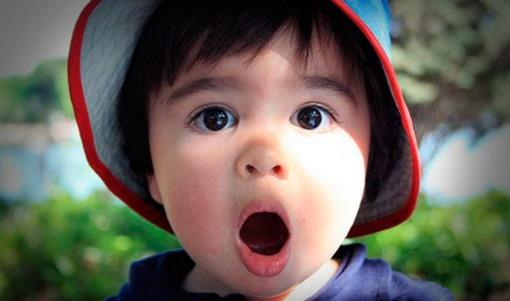
\includegraphics[width=50mm]{./Imagenes/imagen_entrada.png}
		\caption{Ejemplo de una imagen de entrada.}
		\vspace{0.15cm}
		\textit{Fuente: Consuelo Ferrús, http://www.acompasando.org/orar-el-asombro/}
		\label{fig:imagen_entrada}
\end{figure}


\begin{figure}[H]
		\centering
		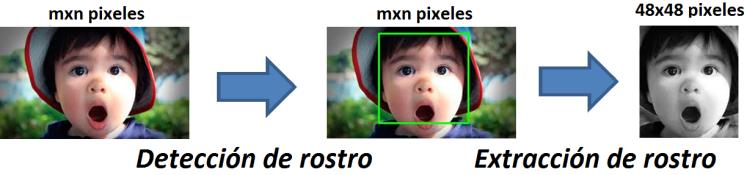
\includegraphics[width=140mm]{./Imagenes/proceso_deteccion.png}
		\caption{Proceso de detección de rostro.}
		\vspace{0.15cm}
		\textit{Fuente: Propio}
		\label{fig:proceso_deteccion}
\end{figure}

Se optó por la utilización del detector de rostros \textit{Haar Cascade}, debido a que este es ampliamente utilizado por el nivel de precisión que posee~\cite{6russakovsky2015imagenet}. Sin embargo, esta técnica aun presenta algunas fallas cuando el rostro presenta algún tipo de oclusión(figura~\ref{fig:oclussion}). Este tipo de problema tambien puede ser solucionado construyendo una red convolucional orientada a la detección o localización de rostros, o por medio de otro tipo de técnicas tradicionales basadas en la extracción de características. Debido al tiempo y bajos recursos computacionales, se opto por proponer este tipo de enfoques como trabajos futuros.

\begin{figure}[H]
		\centering
		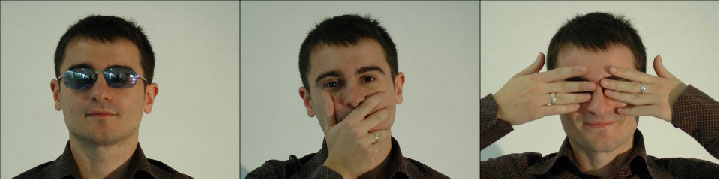
\includegraphics[width=130mm]{./Imagenes/oclussion.jpeg}
		\caption{Ejemplo de rostros con oclusión.}
		\vspace{0.15cm}
		\textit{Fuente: Face Dataset, Universidad Politécnica de Catalunya.}
		\label{fig:oclussion}
\end{figure}

\section{Experimentación en la Elección de Parámetros y Capas en la Construcción de la Arquitectura CNN}

La creación de un modelo depende tanto de la arquitectura (número y orden de las capas de convolucion, capas de Pooling, capas totalmente conectadas, etc.) como de los parámetros de cada capa (número de filtros en la capa de convolucion, tamaño de los filtros, operaciones de agrupación en la capa de submuestreo, etc.).

\textbf{¿Por qué esta configuración de capas y parámetros?} Para la elección de las capas y parámetros, se hizo experimentos con distintas configuraciones en la arquitectura, seleccionando las capas y parámetros da cada una de ellas mediante prueba y error, evaluando el error y precisión de cada configuración.

Se evaluaron 3 arquitecturas con distintas configuraciones de capas y parámetros en las bases de datos FER2013 y CK+.



\begin{itemize}
\item {\textbf{Conv-Conv-Pool-Conv-Conv-Pool-FC}

\begin{table}[H]
    \centering
    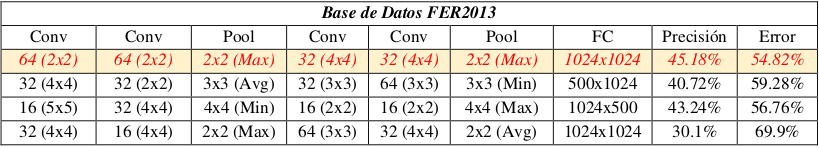
\includegraphics[width=140mm]{./Imagenes/tabla_arqui_1_fer.png} 
    \caption{Evaluación de la arquitectura 1 y sus parámetros, FER2013}
    \label{tab:tabla_arqui_1_fer}
\end{table}

\begin{table}[H]
    \centering
    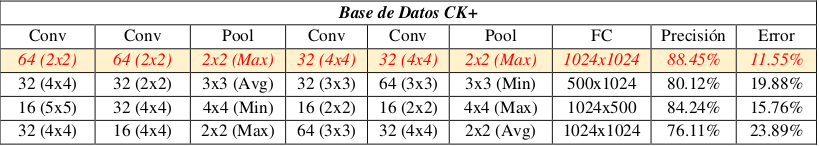
\includegraphics[width=140mm]{./Imagenes/tabla_arqui_1_CK.png}
    \caption{Evaluación de la arquitectura 1 y sus parámetros, CK+}
    \label{tab:tabla_arqui_1_CK}
\end{table}

}

\item {\textbf{Conv-Pool-Conv-Pool-FC \underline{\textit{Arquitectura Propuesta}} }

\begin{table}[H]
    \centering
    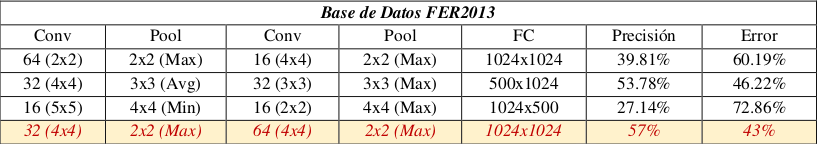
\includegraphics[width=140mm]{./Imagenes/tabla_arqui_2_fer.png} 
    \caption{Evaluación de la arquitectura 2 y sus parámetros, FER2013}
    \label{tab:tabla_arqui_2_fer}
\end{table}

\begin{table}[H]
    \centering
    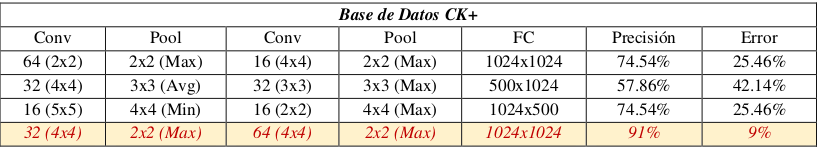
\includegraphics[width=140mm]{./Imagenes/tabla_arqui_2_CK.png}
    \caption{Evaluación de la arquitectura 2 y sus parámetros, CK+}
    \label{tab:tabla_arqui_2_CK}
\end{table}

}

\item {\textbf{Conv-Pool-Pool-Conv-Conv-Pool-FC}

\begin{table}[H]
    \centering
    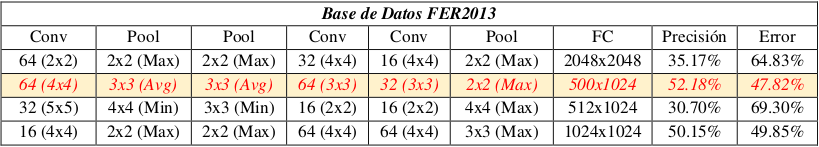
\includegraphics[width=140mm]{./Imagenes/tabla_arqui_3_fer.png} 
    \caption{Evaluación de la arquitectura 3 y sus parámetros, FER2013}
    \label{tab:tabla_arqui_3_fer}
\end{table}

\begin{table}[H]
    \centering
    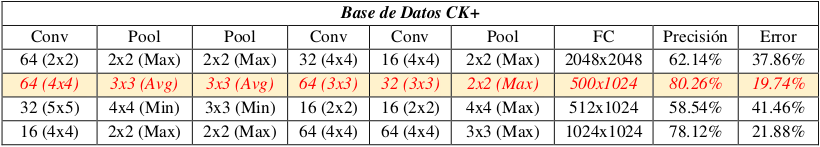
\includegraphics[width=140mm]{./Imagenes/tabla_arqui_3_CK.png}
    \caption{Evaluación de la arquitectura 3 y sus parámetros, CK+}
    \label{tab:tabla_arqui_3_CK}
\end{table}
}

\end{itemize}

\section{Arquitectura Propuesta}
La entrada de nuestra arquitectura consta de una imagen de 48x48 pixeles en
escala de gris que es el resultado de la detección y recorte hecho en la fase de detección
de rostro, seguido de una capa de 32 convoluciones con filtro de 4x4 sin solapamiento,
luego se aplica un sub muestreo de 2x2 con función MAX \footnote[6]{Función que determina el máximo de n números.} , seguido de una capa de 64
convoluciones con filtros de 2x2 sin solapamiento, para posteriormente aplicar un sub
muestreo de 2x2 con función MAX, aplicada las convoluciones y sub muestreo
procedemos a aplicar el Dropout\footnote[7]{Una forma simple de prevenir el \textit{overfitting} en Redes Neuronales..} con 20\%, seguido de dos capas de 1024 neuronas
totalmente conectadas cada una. Finalmente, para la clasificación se aplica la función de
normalización Softmax, que en este proyecto toma 6 clases que representa a las 6
expresiones faciales antes mencionadas.
\vspace{0.5cm}
\begin{table}[H]
    \centering
    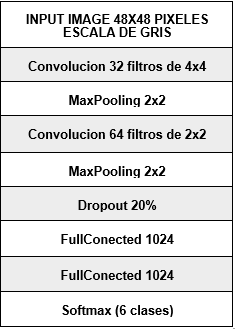
\includegraphics[width=50mm]{./Imagenes/tabla_arquitectura.png}
    \caption{Arquitectura del modelo propuesto}
    \label{tab:tabla_arquitectura}
\end{table}

\section{DESCRIPCIÓN DE LAS CAPAS DE LA ARQUITECTURA}
La arquitectura de Red Neuronal Convolucional sigue la siguiente composición:
\begin{itemize}
\item Primera capa de convolución.
\item Primera capa de Pooling.
\item Segunda capa de Convolución.
\item Segunda capa de Pooling.
\item Primera capa totalmente conectada
\item Segunda capa totalmente conectada
\end{itemize}

\vspace{0.5cm}

\begin{itemize}
\item
{
\textbf{Primera capa convolución.}Cuenta con 32 filtros (mapa de características) del
tamaño 4x4 pixeles. Esta capa tiene la función de extraer las características
relevantes (en el caso de expresiones faciales se puede ver en la Figura 26 que las
características más relevantes son: los ojos, boca, nariz, y otras deformaciones en
el rostro) de la imagen de entrada de tamaño 48x48 pixeles, generando 32 nuevas
imágenes de tamaño 45x45 pixeles a partir de los filtros aplicados.
\begin{figure}[H]
		\centering
		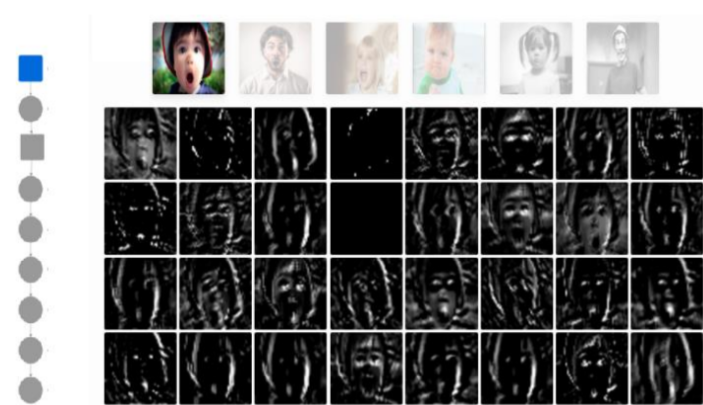
\includegraphics[width=80mm]{./Imagenes/filtro1.png}
		\caption{Imágenes después de la primera convolución.}
		Source: Propia
		\label{fig:filtro1}
\end{figure}
}

\item
{
\textbf{Primera capa de Pooling.}Recibe como parámetros de entrada
las imágenes generadas a partir de la primera capa de convolución. Su función es
la de reducir características redundantes mediante la agrupación de pixeles,
generando 32 nuevas imágenes de tamaño 22x22 pixeles.
\begin{figure}[H]
		\centering
		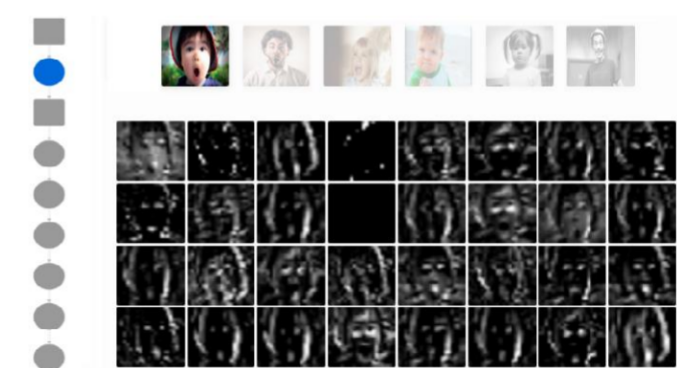
\includegraphics[width=80mm]{./Imagenes/filtro2.png}
		\caption{Imágenes después del primer Pooling.}
		Source: Propia
		\label{fig:filtro2}
\end{figure}
}

\item
{
\textbf{Segunda capa de Convolución.}Cuenta con 64 filtros, recibe como parámetros
de entradas las imágenes generadas a partir de la primera capa de Pooling. Su
función es extraer las características relevantes de las imágenes de entrada,
generando 64 nuevas imágenes de tamaño 21x21 pixeles.
\begin{figure}[H]
		\centering
		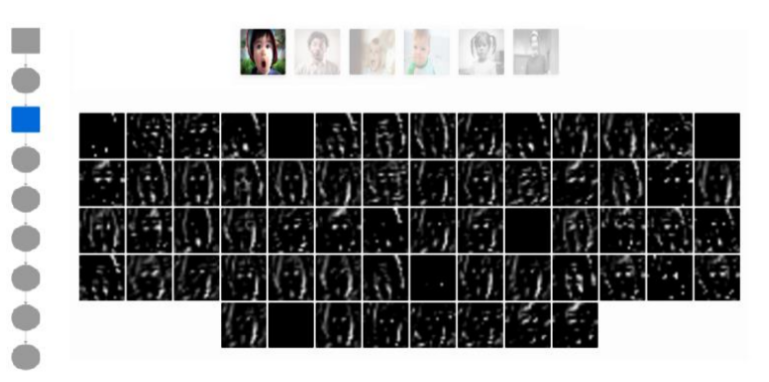
\includegraphics[width=80mm]{./Imagenes/filtro3.png}
		\caption{Imágenes después de la segunda convolución.}
		Source: Propia
		\label{fig:filtro3}
\end{figure}
}

\item
{
\textbf{Segunda capa de Pooling.}Recibe como parámetros de entrada
las imágenes generadas a partir de la segunda capa de convolución. Su función es
la de reducir características de estas imágenes mediante la agrupación de pixeles,
generando 64 nuevas imágenes de tamaño 10x10 pixeles.
\begin{figure}[H]
		\centering
		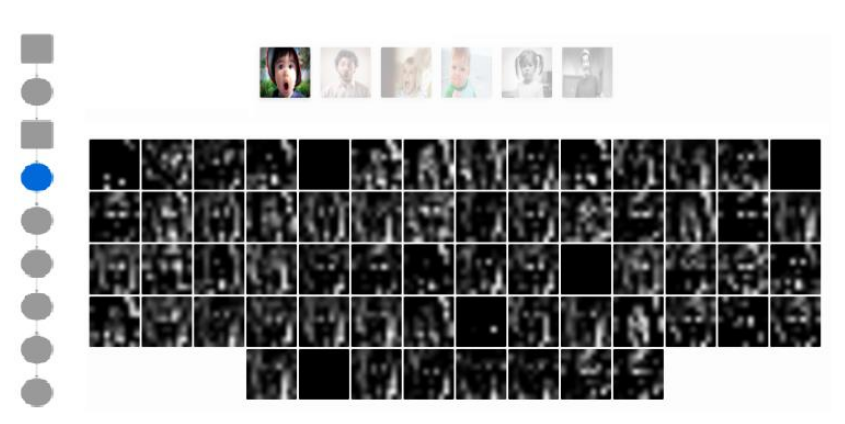
\includegraphics[width=80mm]{./Imagenes/filtro4.png}
		\caption{Imágenes después del segundo Pooling.}
		Source: Propia
		\label{fig:filtro4}
\end{figure}
}
\item
{
\textbf{Capas totalmente conectadas.}
Recibe como parámetros de entrada las imágenes
generadas a partir de la segunda capa de Pooling, su función es la de ajustar los
pesos en las conexiones de las neuronas pertenecientes a la arquitectura,
minimizando el error haciendo uso del algoritmo BackPropagation. La última
capa totalmente conectada cuenta con 6 neuronas, las cuales representan las 6
expresiones faciales utilizadas en este proyecto.
}
\end{itemize}

\section{PARAMETROS DE LA ARQUITECTURA}
La imágenes de entrada son definidas en el tamaño de 48x48 píxeles como valor
estándar basándonos en el tamaño en el cual están las imágenes de la base de datos
FER2013, el número de convoluciones en la primera capa es de 32 y 64 en la segunda
capa de convolución obteniendo así un total de 32x64 mapas de características, la capa
de Pooling agrupa subregiones de las dimensiones 2x2 píxeles para que no se pierda
mucha información, nosotros optamos por la elección de dos capas totalmente conectadas
de 1024x1024 producto de los resultados obtenidos basándonos en prueba y error , el total
de parámetros obtenidos con la arquitectura propuesta es de:

\begin{itemize}
\item Imagen de entrada: 48x48 píxeles
\item 1ra capa con 32 convoluciones: 544 parámetros
\item 2da capa con 64 convoluciones: 8256 parámetros
\item 1ra capa totalmente conectada: 6554624 parámetros
\item 2da capa totalmente conectada: 1049600 parámetros
\item función de normalización Softmax: 7175 parámetros
\end{itemize}
Obteniendo un total de 7,620,199 parámetros totales.

\begin{table}[H]
    \centering
    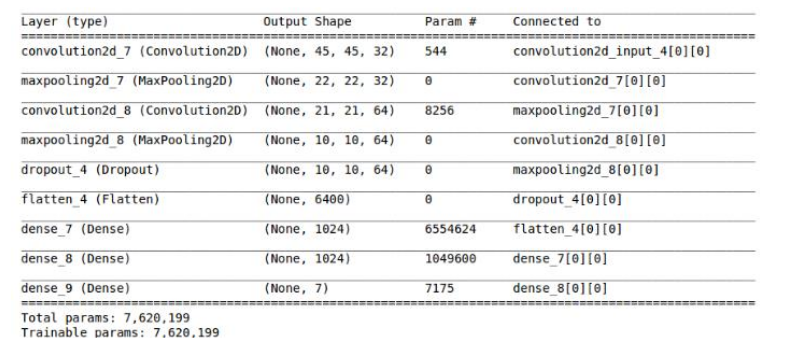
\includegraphics[width=140mm]{./Imagenes/parametros.png} 
    \caption{Número de parámetros de nuestra CNN}
    \label{tab:parametros}
\end{table}


\begin{figure}[H]
		\centering
		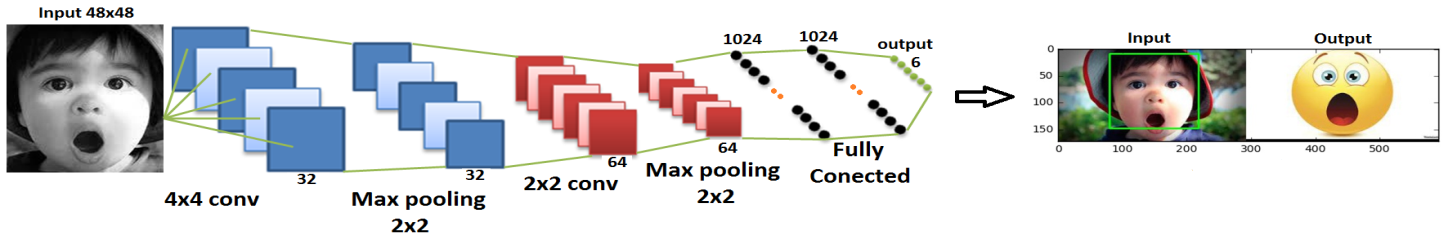
\includegraphics[width=180mm]{./Imagenes/arquitectura_CNN_grafico.png}
		\caption{Arquitectura grafica del modelo propuesto}
		Source: Propio
		\label{fig:arquitectura_CNN_grafico}
\end{figure}
	
\section{ENTRENAMIENDO DE LA CNN}
El entrenamiento de nuestra Red Neuronal Convolucional siguió un proceso
iterativo en el que se presentó como datos de entrada imágenes de expresiones faciales y
sus respectivas etiquetas de salida (clases correspondientes a la expresión facial a la cual
pertenece: enojo, miedo, alegría, tristeza, sorpresa y neutro).

Durante esta fase de entrenamiento, la Red Neuronal Convolucional aprendió
mediante el ajuste de sus pesos, con el fin de ser capaz de predecir la etiqueta de clase
correcta de los datos de entrada, el algoritmo de Red Neuronal más popular para la fase
de entrenamiento es el algoritmo de BackPropagation, dicho algoritmo se usó en nuestra
fase de entrenamiento. Los pesos iniciales de nuestra red se eligieron al azar y comienza
el entrenamiento o aprendizaje. Se procesó los datos de entrada para lograr obtener las
etiquetas deseadas obteniendo un error el cual se propago hacia atrás mediante el
algoritmo antes mencionado(BackPropagation) haciendo que se ajusten los pesos, este
proceso ocurrió una y otra vez hasta que se minimizo el error y eso ocurrió cuando se
logró una convergencia de los datos.

\section{TEST AL MODELO CREADO}
Una vez creada el modelo (un archivo con extensión .h5) se procede a realizar las
consultas a dicho modelo, estas consultas siguen los siguientes pasos:

\begin{itemize}
\item Leer una imagen de entrada, de dimensiones mayos o igual a 48x48 pixeles.
\item Utilizar Haar Cascade para la detección del rostro en la imagen antes ingresado.
\item Extraer el rostro detectado y redimensionarlo al tamaño 48x48 pixeles.
\item Dar como imagen de entrada la imagen obtenida en el paso anterior.
\end{itemize}
Después de realizar los pasos anteriores, el modelo arrojara un valor asociado a la
expresión facial predicha.

\section{RECOPILACIÓN DE IMAGENES DE EXPRESIONES
FACIALES}
La recopilación de las imágenes de expresiones faciales se obtuvo de 2 fuentes
secundarias de información (internet) en los cuales los datos están pre-elaborados
(imágenes con tamaños de 48x48 pixeles de base de datos FER20131 y 640x490 o
640x480 píxeles de la base de datos CK+).

\section{BASE DE DATOS}
Se usó 3 bases de datos ($FER2013^{1}$ y $CK+^{2}$ ) y una tercera como resultado de la
unión de las 2 bases de datos antes mencionadas.
\subsection{FER2013}
Es una base de datos del sitio web Kaggle{1} para el concurso de reconocimiento de
expresiones faciales.

Esta base de datos posee 35887 imágenes en escala de gris de 48x48 pixeles,
clasificados en 7 categorías (enojado, disgustado, miedo, feliz, triste, sorpresa y neutro).
En este trabajo se optó por unir la categoría enojado y disgustado por las similitudes que
tienen entre ellas.

Separamos la data en 2 partes training y test. El training consta de 32298 imágenes
y el test de 3589 imágenes.

\begin{figure}[H]
		\centering
		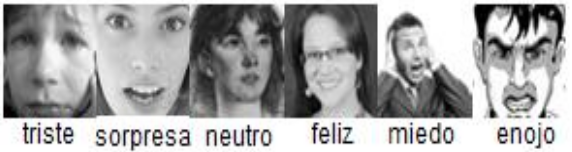
\includegraphics[width=90mm]{./Imagenes/imagenes_fer.png}
		\caption{Imágenes de la base de datos FER2013}
		Source: Kaggle
		\label{fig:imagenes_fer}
\end{figure}

\section{CK+}
La base de datos $CK+^{2}$ (Cohn-Kanade) posee imágenes de expresiones faciales
frontales de 210 personas en resolución de 640x490 o 640x480 pixeles. Nosotros
elegimos de entre ellos 3289 imágenes convirtiéndolos a escala de gris de 48x48 pixeles
y clasificándolos en 6 categorías (enojado, miedo, feliz, triste, sorprendido y neutro).
Nuestro training consta de 2966 imágenes y el test de 323 imágenes.

\begin{figure}[H]
		\centering
		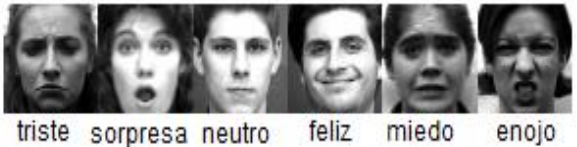
\includegraphics[width=90mm]{./Imagenes/imagenes_ck+.png}
		\caption{Imágenes de la base de datos CK+}
		Source: Base de datos CK+
		\label{fig:imagenes_ck+}
\end{figure}


\section{FER2013 - CK+}
Esta base de datos resulta de la unión de la base de datos Fer2013 y CK+,
obteniendo un total de 39176 imágenes de 48x48 en escala de gris. El training tiene 35264
y el test 3912 imágenes.

\section{RESULTADOS EXPERIMENTALES}
A continuación, se muestra los resultados que se obtuvieron en las diferentes bases
de datos FER2013, CK+ y la tercera base de datos que se obtuvo como resultado de la
unión de los dos antes mencionadas.

Se podrá apreciar los niveles de precisión alcanzado por cada categoría –
Expresión Facial (Enojado, Miedo, Feliz, Triste, Sorprendido, Neutro). Así como sus
matrices de confusión que nos mostraran los resultados positivos y sus falsos positivos,
pudiendo así interpretar de mejor manera los resultados.

\subsection{FER2013}

\begin{table}[H]
    \centering
    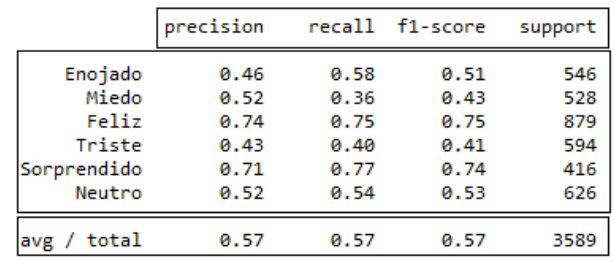
\includegraphics[width=80mm]{./Imagenes/tabla_resultados_fer.png} 
    \caption{Resultados obtenidos - FER2013}
    \label{tab:tabla_resultados_fer}
\end{table}

En la Tabla 3 se puede apreciar los niveles de precisión en la clasificación de los
datos de la base de datos FER2013, mostrando en la categoría Enojado 46\%, Miedo 52\%,
Feliz 74\% Triste 43\%, Sorprendido 71\% y Neutro 52\%.

\begin{figure}[H]
		\centering
		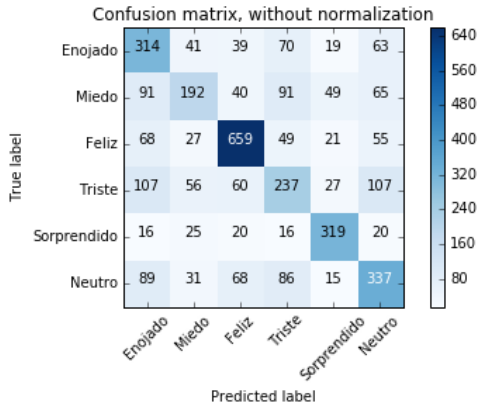
\includegraphics[width=80mm]{./Imagenes/matriz_confusion_fer.png}
		\caption{Matriz de confusión, precisión del Test - FER2013}
		\label{fig:matriz_confusion_fer}
\end{figure}

\begin{figure}[H]
		\centering
		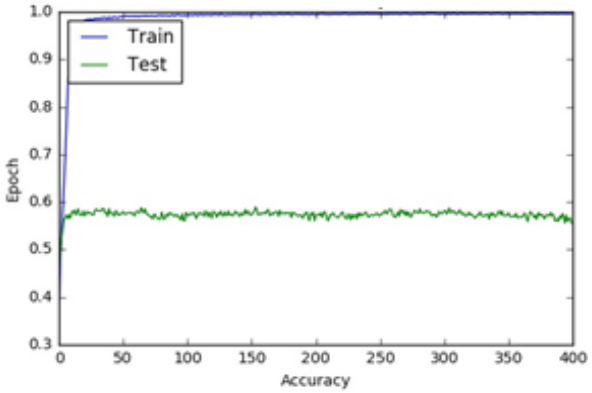
\includegraphics[width=80mm]{./Imagenes/precision_fer.png}
		\caption{Precisión durante el proceso de entrenamiento y prueba (\%) – FER2013}
		\label{fig:precision_fer}
\end{figure}

\begin{figure}[H]
		\centering
		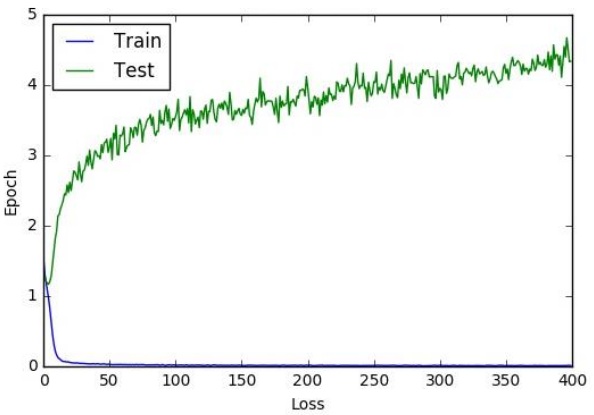
\includegraphics[width=80mm]{./Imagenes/perdida_fer.png}
		\caption{Perdida durante el proceso de entrenamiento y prueba (\%) – FER2013}
		\label{fig:perdida_fer}
\end{figure}

\subsection{CK+}

\begin{table}[H]
    \centering
    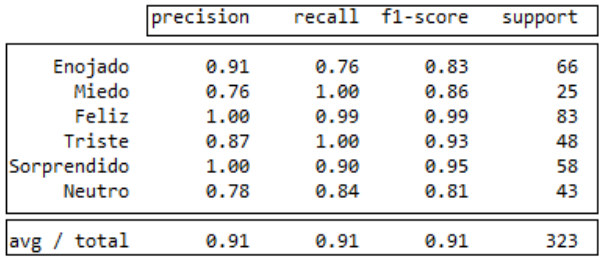
\includegraphics[width=80mm]{./Imagenes/tabla_resultados_ck+.png} 
    \caption{Resultados obtenidos - CK+}
    \label{tab:tabla_resultados_ck+}
\end{table}

En la Tabla 4 se puede apreciar los niveles de precisión en la clasificación de los
datos de la base de datos CK+, mostrando en la categoría Enojado 91\%, Miedo 76\%,
Feliz 100\%, Triste 87\%, Sorprendido 100\% y Neutro 78\%.

\begin{figure}[H]
		\centering
		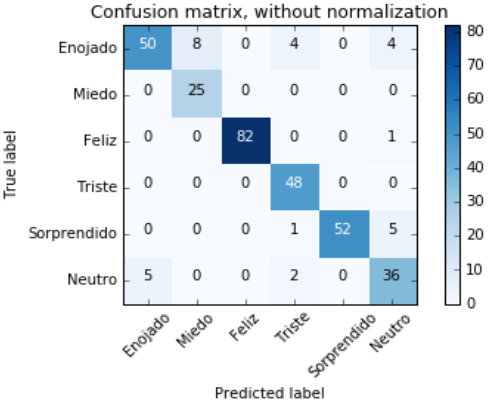
\includegraphics[width=80mm]{./Imagenes/matriz_confusion_ck+.png}
		\caption{Matriz de confusión, precisión del Test - CK+}
		\label{fig:matriz_confusion_ck+}
\end{figure}

\begin{figure}[H]
		\centering
		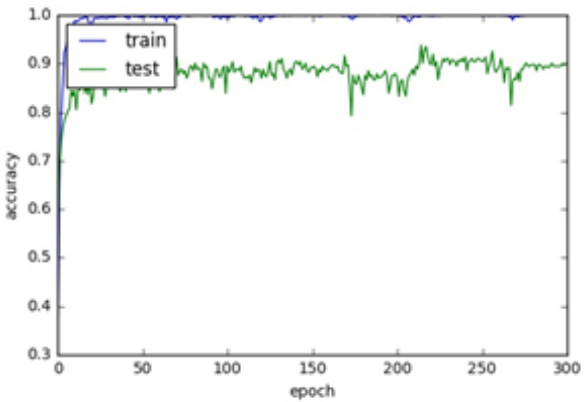
\includegraphics[width=80mm]{./Imagenes/precision_ck+.png}
		\caption{Precisión durante el proceso de entrenamiento y prueba (\%) - CK+}
		\label{fig:precision-ck+}
\end{figure}

\begin{figure}[H]
		\centering
		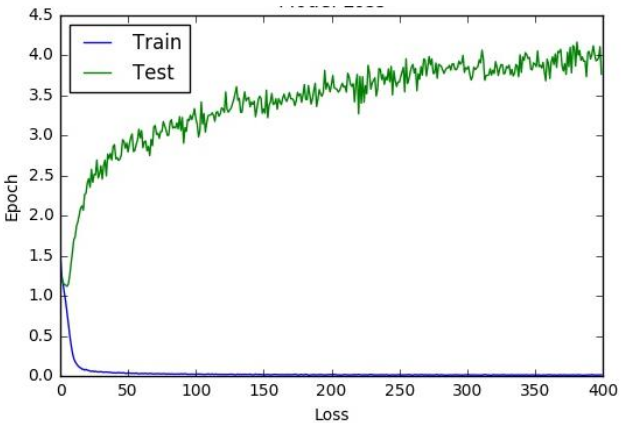
\includegraphics[width=80mm]{./Imagenes/perdida_ck+.png}
		\caption{Perdida durante el proceso de entrenamiento y prueba (\%) – FER2013}
		\label{fig:perdida_ck+}
\end{figure}

\subsection{FER2013 - CK+}


\begin{table}[H]
    \centering
    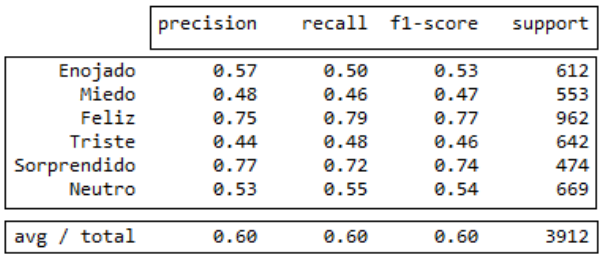
\includegraphics[width=80mm]{./Imagenes/tabla_resultados_fer_ck+.png} 
    \caption{Resultados obtenidos - FER2013 - CK+}
    \label{tab:tabla_resultados_fer_ck+}
\end{table}

En la Tabla 5 se puede apreciar los niveles de precisión en la clasificación de los
datos de la base de datos (FER2013 - CK+), mostrando en la categoría Enojado 57\%,
Miedo 48\%, Feliz 75\%, Triste 44\%, Sorprendido 77\% y Neutro 53\%

\begin{figure}[H]
		\centering
		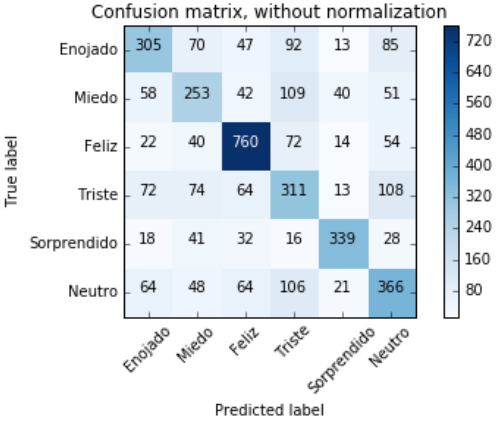
\includegraphics[width=80mm]{./Imagenes/matriz_confusion_fer_ck+.png}
		\caption{Matriz de confusión, precisión del Test FER2013 - CK+}
		\label{fig:matriz_confusion_fer_ck+}
\end{figure}

\begin{figure}[H]
		\centering
		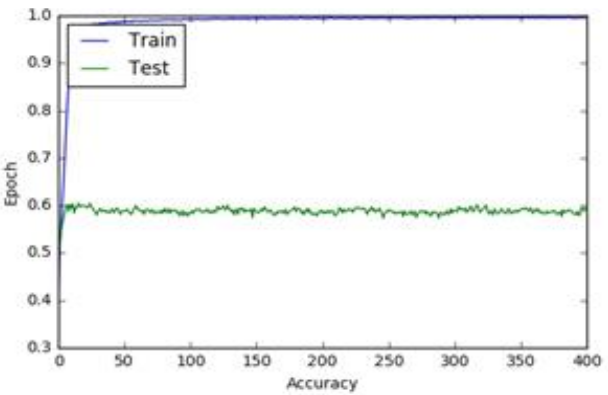
\includegraphics[width=80mm]{./Imagenes/precision_fer_ck+.png}
		\caption{Precisión durante el proceso de entrenamiento y prueba (\%) FER2013 - CK+}
		\label{fig:precision_fer_ck+}
\end{figure}

\begin{figure}[H]
		\centering
		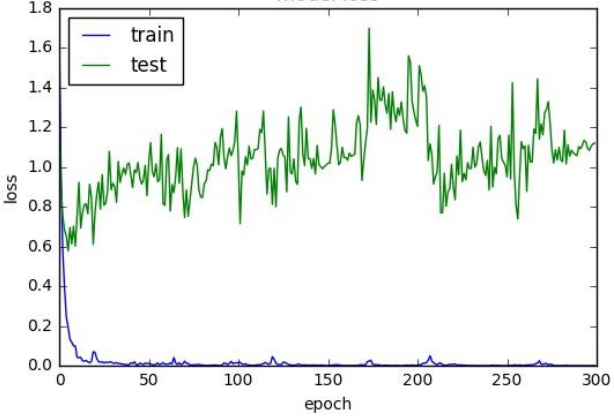
\includegraphics[width=80mm]{./Imagenes/perdida_fer_ck+.png}
		\caption{Perdida durante el proceso de entrenamiento y prueba (\%) FER2013 - CK+}
		\label{fig:perdida_fer_ck+}
\end{figure}


